\documentclass{IEEEtran}

\usepackage[utf8]{inputenc}
\usepackage[english]{babel}
\usepackage{graphicx}
%\usepackage[margin = 1in]{geometry}
 
\usepackage{biblatex}
\addbibresource{sources.bib}

\title{ET4394 Wireless Networking - Analyzing 802.11 CRC faults}
\date{\today}
\author{
Bart Rijnders - 4103505 \\
Bernard Bekker - 4221656 
}

\begin{document}

\maketitle

\begin{abstract}

In this report the effect of signal strength, frequency and data rate on the amount of CRC failures in WiFi networks is analyzed. Data is gathered using a laptop 801.11 PHY. Our results show an increasing amount of CRC errors at lower signal strength, a lower maximum datarate at a lower signal strength and no strong relation between packet length and airtime and CRC errors. 
\end{abstract}

\section{Hypotheses}

Packet loss can occur when the signal to noise ratio is insufficiently high to sustain communication at a certain datarate, or when two WiFi packets collide \cite{4509719}. Based on this, we expect to see several relations between characteristics of the packets being received, and their error rates:

\subsection{Signal to noise ratio}
We expect to see a quick drop off when the signal-to-noise ratio drops below the required SNR value to have a reliable link.

\subsection{Packet length}
Since the chance of a bit error occurring is equal for each bit in the packet. We expect the chance of a CRC error to follow $P(biterror)^{length}$. 

\subsection{Used frequency/channel}
We expect to see a difference in errors on different channels, based on their frequency and depending on how busy they are.

\subsection{Packet datarate}
We expect to see a higher amount of errors when seeing a low signal combined with a high datarate. For a consistent signal strength, a lower datarate should result in less errors. However, this can result in a higher chance of collisions as airtime increases \cite{4215626}. 

\section{Methodology}

WiFi packets are captured on a laptop using an intel wireless dualband-AC 8265 network adapter. Other methods attempted to capture packets include an Alfa awus036ac external wifi adapter, and a C.H.I.P. ARM devboard with build in wifi. The network adapter was placed in monitor mode using the airmon-ng application, and TShark was used to capture only data packets. A python script was written for changing the channel every 5 seconds. Approximately 1M packets are captured in lecture halls, and 1M packets in a flat building. All data is processed in Python using pandas and matplotlib.


\section{Results}

\subsection{Signal strength versus CRC errors}

Some interesting aspects can be seen in figure \ref{fig:totalpackets}. The good reception at high signal strengths, a strong dropoff after a certain point, and two main dips in the reception of correct packets. The most startling aspect is the rise in correctly received packets at even lower signal strength. We can see more patterns if we split the results into 2.4Ghz channels, and 5.8 Ghz channels (fig \ref{fig:24packets} and fig \ref{fig:58packets}). The two dips are explained by the different dropoff points for 2.4 Ghz and 5.8Ghz. Because the 5.8Ghz has less noise due to concrete walls shielding interfering signals, the packets can be correctly demodulated at a lower signal strength.

\begin{figure*}[tb]
		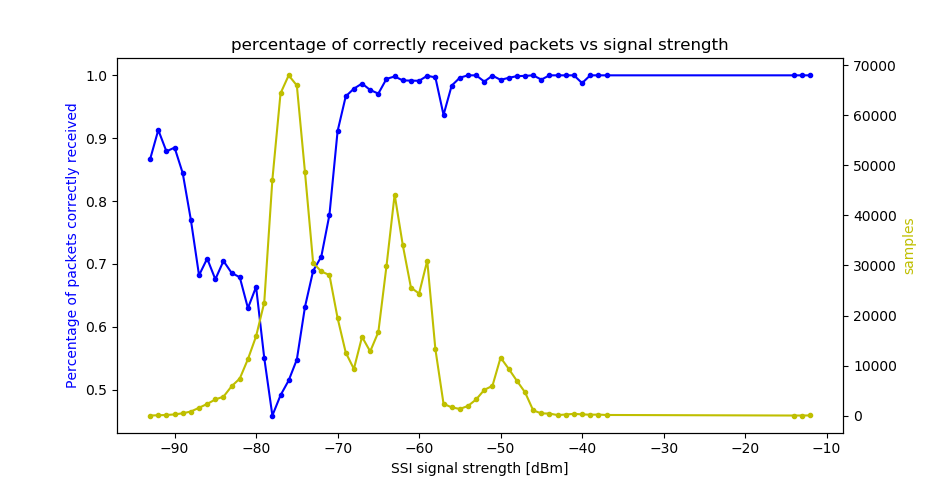
\includegraphics[width=\textwidth]{figures/packets_total.png}
		\caption{A total overview of CRC error rates in packets versus signal strength. The blue line shows the portion of messages being received without a CRC error. The yellow line show the amount of samples at each data point. }
		\label{fig:totalpackets}
\end{figure*}

\begin{figure}
		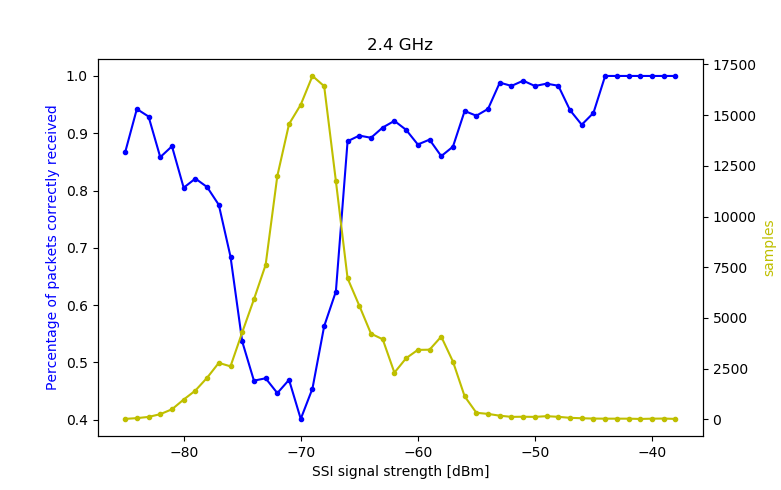
\includegraphics[width=0.5\textwidth]{figures/24ghz.png}
		\caption{correctly received packets versus signal strength for packets send on the 2.4Ghz frequency.}
		\label{fig:24packets}
\end{figure}

\begin{figure}
		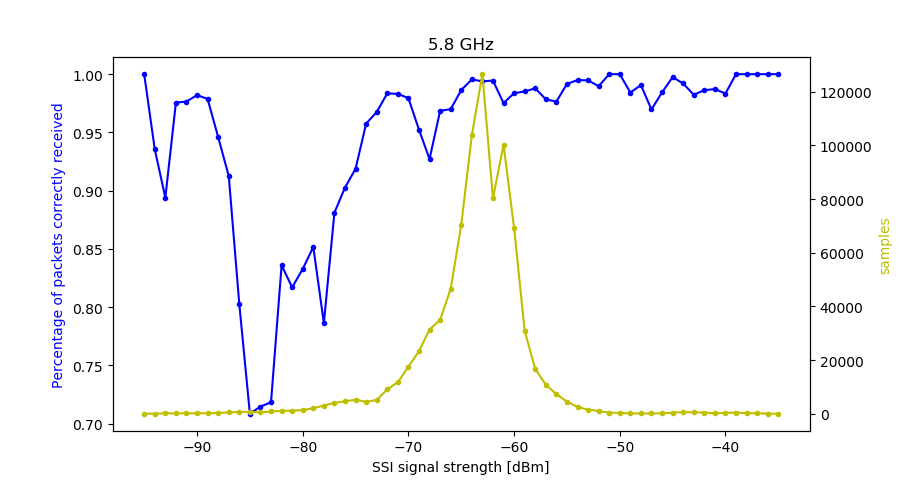
\includegraphics[width=0.5\textwidth]{figures/58ghz.png}
		\caption{correctly received packets versus signal strength for packets send on the 5.8Ghz frequency.}
		\label{fig:58packets}
\end{figure}

This leaves to explain why the graph turns up again at very low signal strengths. We expect this to be a result of this experiment being a field experiment. Since we do not have a control of what packets are being send, the packets captured are a mix of different data-rates based on the RSSI of the connection between the devices we are eavesdropping (due to adaptive data rates). The results only show the packets that are received by the network adapter used in this experiment. When the signal deteriorates too far, packets are no longer forwarded to the driver and OS. We can see this clearly in fig \ref{fig:datasignal}: At low signal strengths, only the packets with a low datarate are decoded by our PHY (As expected due to Shannon's law). This implies that we should see a traditional curve when we isolate a single datarate, and this is confirmed in fig \ref{fig:singledatarate}.

\begin{figure*}
		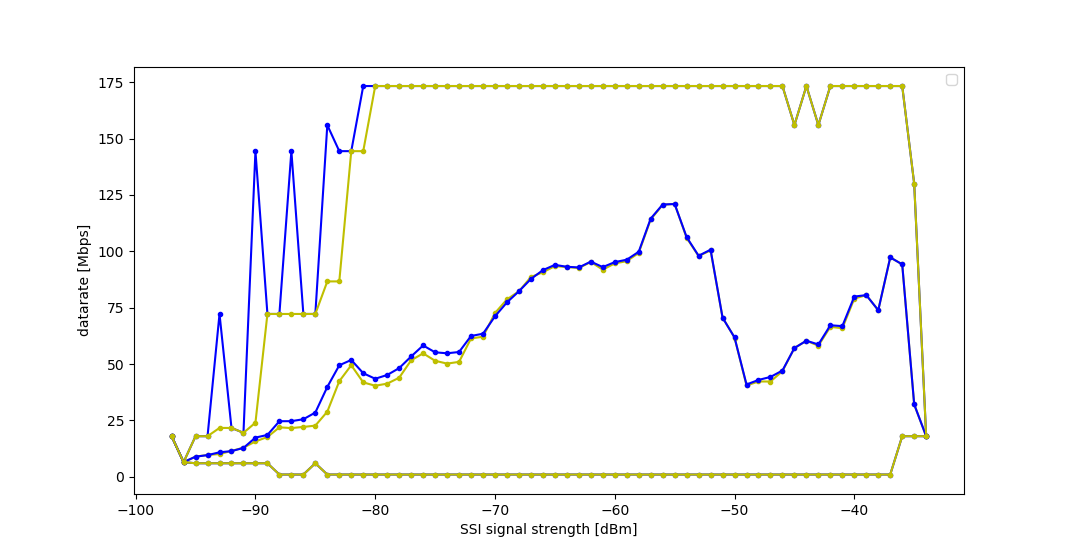
\includegraphics[width=\textwidth]{figures/datarate_signal.png}
		\caption{maximum, mean and minimal reported datarates of received packets vs. signal strength. The blue line is the datarate of all received packets, the green line the datarate of packets without CRC errors. The difference between the average datarate of all and only successful packets represents the amount of errors due to using a too high datarate. At low signal strengths, all lines converge as the network adapter drops all undecipherable packets and only shows packets that are successfully received due to their low datarate.}
		\label{fig:datasignal}
\end{figure*}

\begin{figure}
		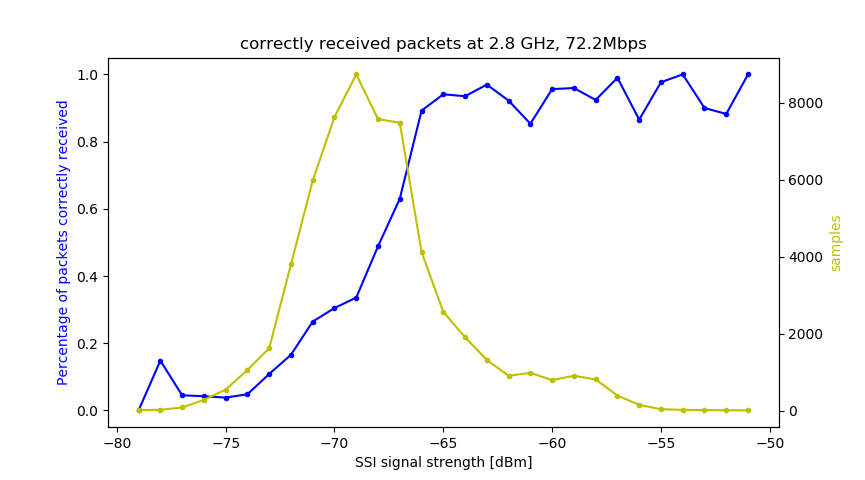
\includegraphics[width=0.5\textwidth]{figures/24ghz72mbps.png}
		\caption{correctly received packets versus signal strength for packets send on the 2.4Ghz frequency with a datarate of 72Mbps.}
		\label{fig:singledatarate}
\end{figure}

\subsection{Packet length}

Contrary to our expectations, the relation between packet length and the error percentage seems not to be exponential. No clear correlation could be found using the least-squares method. This can be explained by the devices communicating adapting the settings of the channel to keep the error rate low. In the prior work \cite{7317401}, the authors saw a constant error rate with increasing packet length, but an increase in error rate when increasing the airtime. However, this seemed mostly constant in our datasets (see fig \ref{fig:airtime}). 

\begin{figure}
		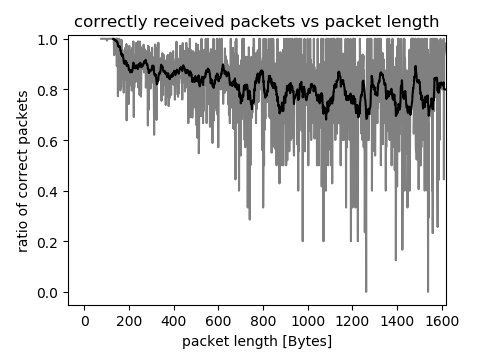
\includegraphics[width=0.5\textwidth]{figures/length.png}
		\caption{Percentage of packets without error versus packet length.}
		\label{fig:length}
\end{figure}

\begin{figure}
		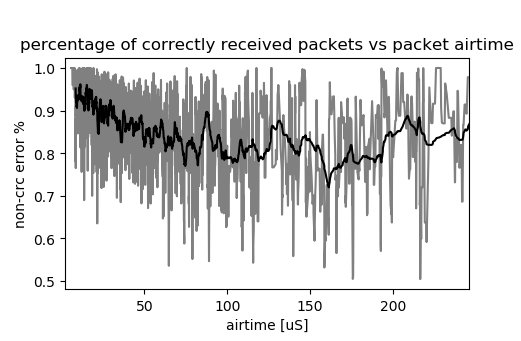
\includegraphics[width=0.5\textwidth]{figures/airtime.png}
		\caption{Percentage of packets without error versus airtime. Gray line showing the raw data, and black line filtered using a rolling window filter of size 50. (Calculated using packet length in bits / packet datarate in Mbps)}
		\label{fig:airtime}
\end{figure}


\subsection{Channels}
\begin{table}[h]
\centering
\caption{packet success rate in a flat building}
\label{tbl1}
\begin{tabular}{lll}
Channel & \% successful packets & Samples \\
1       & 98\%                          & 352763  \\
5       & 52\%                         & 277195  \\
6       & 67\%                          & 99189   \\
9       & 100\%                           & 3237    \\
44      & 100\%                           & 415    
\end{tabular}
\end{table}

\begin{table}[h]\centering
\caption{packet success rate in a university lecture hall}
\label{tbl2}
\begin{tabular}{lll}
Channel & \% successful packets & Samples \\
1       & 96\%                          & 352763  \\
5       & 52\%                          & 277195  \\
9       & 84\%                          & 99189   \\
44      & 99\%                          & 3237   \\
48      & 80\%                          & 415    \\
60      & 95\%                          & 1425   \\
100     & 96\%                          & 137178 \\
\end{tabular}
\end{table}

Tables \ref{tbl1} and \ref{tbl2} show the measured CRC error rates for different channels. A proper analysis of the effects of the different channels requires more data points at more locations and times. But at least at the locations that were measured, channel 5 seems to be a channel to avoid!

\subsection{Packet datarate}
Our data shows few CRC errors for both high and low datarates at high signal strengths (fig \ref{fig:datasignal}). At critical signal strengths, the average datarate of packets without an error is slightly lower than for all packets. At low signal strength, only packets with a low datarate are received by the network adapter. This is consistent with our expectations.

\section{Discussion}
Our experiments not only measured the effects of fundamental wireless networking theory, but also the techniques used by devices to optimize their reception and what packets are reported to the OS. We have seen the effects of adaptive datarates, adaptive packet lengths, and adaptive power control. This can often result in unexpected data if not all variables are corrected for.  

Our ability to get good results was hindered by the capabilities of our hardware. We were not able to perform an experiment in an controlled situation, and could not quantify the noise floor during our measurements. For some reason, our capturing laptop completely ignored some packets send by some devices, but did show others. If this effect is random, it should not have affected the result shown here. But since we could not fully control for all the effects, we can't be sure.


\printbibliography

\end{document}